%2.1 [0 Journal Articles Used]
\section{Introduction}
\paragraph{}
The overall use of handheld devices has undoubtedly increased astronomically within the past decade or so. Various resources and connecting with others around the world has been made easily accessible to those with such devices. To a great extent, this eliminates the factor of distance for such individuals. As it is evident, the past nearly two years have forced us into an era and lifestyle of isolation. COVID-19's impacts on everyone has pushed apart families, friends, and colleagues making it quite difficult to stay connected, especially in person. The internet, social media, Facetime, Zoom, and numerous other mobile applications and websites have all aided our world with the capability to stay connected with each other, but separately. As we continue through this period of seclusion, many advancements for staying connected have blossomed. Zoom Video Communications, used to host virtual meetings for any occasion, for example, has skyrocketed in its usage. At Worcester Polytechnic Institute, the same ideals hold true. So, we took on the challenge to join this movement and develop a mobile application tailored to the utilization of the George C. Gordon Library's many resources. In doing so, like the other platforms mention previously, it would allow users to connect to the library's resources remotely and follow local COVID-19 guidelines with the additional provided information about the library and its in-person availabilities within the app.

%2.2 [7 Journal Articles Used]
\section{Significance of the Topic}
\paragraph{}
 Our world is becoming more and more reliant on devices such as our mobile phones. These mobile devices unlock a connection between the user and a vast and seemingly endless supply of helpful and sometimes not so helpful resources. With this in mind, this connective architecture "serves as a virtual platform for learners to engage with their learning activities in a more spontaneous, personal, informal, contextual, portable, ubiquitous and pervasive way", as \textit{Adoption of mobile library apps as learning tools in higher education: a tale between Hong Kong and Japan} explains \cite{Mobile_Apps_Between_Hong_Kong_and_Japan}. Mobile applications have become and are continuing to be greatly utilized in the academic world on all levels. From children to college graduate students, technology aids each one to some extent, broadening their learning capabilities and resources. When someone hears "mobile application" or "app" they typically think of a major application they often utilize. However, there are "a considerable number of apps are very small in size and sometimes tends to follow no particular design principle" \cite{Challenges_in_Mobile_Apps}. Mobile apps can often emulate desktop - based websites, but are streamlined in comparison. The use of this is to take a website that is accessable through a desktop or laptop and enable the same or more stark access to the same website. As developing a mobile website that could house the resources of a library may be a more simple task, it leaves for less capabilities and utilities for the mobile user. Developing a native application that can support all mobile platforms is more daunting, but a much higher quality product in the end. The user experience in this case is far superior to a mobile website \cite{misodi}.
 
\paragraph{}
 In his article \textit{Undergraduate students use of mobile apps to search library catalogs} Shih-Chuan Chen states, based on the results from a survey constituted on undergraduate students, that "Many libraries provide mobile app services because of the rapid increase in smartphone users" \cite{undergrad_ma}. He also goes on to note how many elementary tasks are accomplished more efficiently on a mobile device than on a computer, however, the inverse is true for tasks that require the use of searching and web browsing. Laptops and desktops alike were proven to supersede mobile devices in this case, however, mobile devices are still useful in this aspect \cite{undergrad_ma}. From the results of this survey, having academic options such as mobile resources that are engaging and user friendly could disallow the necessity of in-person attendance to a library or other academic facility. Additionally, in our case with the ongoing pursuit of the Corona Virus, this could reduce the number of people in the library at a given time and allow for a more safe environment as students collectively stay separate. Certain resources such as occupancy tracking, tech suite booking, library hours, and others would not only help students to use their time more efficiently and follow local guidelines in a more safe manner, but also help slow the spread of COVID-19. After all, "we live in a world where convenience is key" \cite{mob_ph_app_aca_lib}. No one of us desires to wait for access to something we need to use. It is a natural human behavior. Technology has amplified that mentality as it provides its users relatively instant access to just about anything at anytime. 

\paragraph{}
When developing a mobile application, many factors have to be considered well in advance before code starts to be structured and written. For example, a native application is typically developed to be supported on a specific device platform such as Apple devices. Thus, when developing a mobile app, additional steps need to be taken to include the possibility of the app to be supported by all or most mobile devices. After development, the application will need to be verified and reviewed by the various app stores, i.e. Android's Google Play Store and Apple's App Store, to be displayed and downloadable for any user on each. Since the application is intended to be public and accesable by many, it has to be run on a network server \cite{Mobile_App_Paradigms}. App stores' usages have skyrocketed where, fascinatingly, "[t]he number of apps in both Apple App Store and Google Play [Store] has surpassed the two million mark in 2016 and billions of downloads [6, 20], which makes mobile apps a [major] industry. Recent studies [4, 44] reported that the global mobile app revenues amounted to 41.1 billion US dollars in 2015 and the app economy could double in size to more than 100 billion dollars by 2020. At the same time, the latest estimates [32] indicate that there are 12 million mobile app developers worldwide, representing more than half of the total community, and almost half of app developers focus their attention on the Android platform, which makes mobile app market a very competitive environment. A large mount of research work have focused on the mobile app ecosystem" \cite{Mobile_App_Ecosystem}.

\paragraph{}
Acknowledging the features a mobile application should embody can be relatively easy, but determining the delivery format and final product in which the user consumes such an app is far more difficult. In a study conducted by Ngu Phuc Huy from Norwegian University of Science and Technology and Do vanThanh from Telenor & Norwegian University of Science and Technology, they analyzed four different types of mobile app paradigms namely: Mobile native applications, Mobile widgets, Mobile Web applications, and HTML5 mobile applications. From their research, Ngu Phuc Huy and Do vanThanh devised what they called an "Evaluation Criteria" as exhibited below: \cite{Mobile_App_Paradigms}


\noindent\textbf{EVALUATION CRITERIA:}

\noindent In order to really assert which mobile application paradigms are better it is necessary to consider the viewpoints of all the involved players, namely developer, user and service provider. We deduced the evaluation criteria as follows:

\begin{itemize}
    \item\textbf{Developer's viewpoint:}

    \begin{itemize}
        \item \textbf{Ease of developing:}
        
            \begin{itemize}
                \item \textbf{Programming language:} This sub-criterion tells both about the simplicity and the popularity of the programming language.
                \item \textbf{Software Development Kit (SDK):}
                
                    \begin{itemize}
                        \item \textbf{Applicability:} This sub-criterion relates the applicability and accessibility of the SDK.
                                \item \textbf{Specifications and tips: }This sub-criterion is about the quality of documents accompanied with the SDK.
                                \item \textbf{Download installation and configuration:} These sub-criterion shows how straightforward to download install and configure the SDK on our development environment.
                            \end{itemize}
                            
                            \item\textbf{Support from community:} Thus sub-criterion is about how much help developers could receive from community (e.g. tutorials, development tools and troubleshooting).
                        \end{itemize}
                        
                        \item\textbf{Ease of coding:}
                        \begin{itemize}
                        \item\textbf{IDE capability:}
                        \begin{itemize}
                            \item\textbf{Code editor:} This sub- criterion is about the qualification of the IDE adopted for the app development. A good code IDE will provide immediate feedback with error messaged and warnings, quick fix feature, content assistant and a good guidance document.
                            \item\textbf{User interface builder:} This sub-criterion shows how robust the adopted user interface builder is. A powerful user interface builder will have instantly viewable and drag-and-drop capabilities, and other features reducing the workload of developers to create an attractive user interface.
                        \end{itemize}
                        
                            \item\textbf{User interface:} This sub-criterion shows how straightforward it is to build an attractive and adaptive user interface.
                            \item\textbf{Device’s interaction:}
                            \begin{itemize}
                                \item\textbf{Hardware:} This sub-criterion describes how easy it is to access device’s hardware, such as camera, storage and WLAN card.
                                \item\textbf{Built-in apps:} This sub-criterion shows how effective it is to adopt different built-in apps on devices, such as camera, phonebook and photo gallery apps
                            \end{itemize}
                            
                            \item\textbf{Web service interaction:} This sub-criterion is to evaluate the ease of using a Web service, such as Google Map, Facebook and IQEngine.
                        \end{itemize}
                        
                        \item\textbf{Ease of debugging:} This sub-criterion tells about how powerful and applicable the debugging tools are. A robust debugging tool will help manage break point, trace object value through the code and identify unexpected bugs.
                        \item\textbf{Ease of testing:}
                        
                        \begin{itemize}
                            \item\textbf{Emulator:} This sub-criterion show how effective is the testing of apps on an emulator. A powerful emulator will run fast and support as many device’s features as possible, such as GPS, camera, and accelerator.
                            \item\textbf{Real device:} This sub-criterion show how easy is the testing of apps on a real device.
                        \end{itemize}
                        
                        \item\textbf{ Ease of deploying and updating:} This criterion relates how straightforward it is to deploy and update an app onto a real device.
                        \item\textbf{Ease of distribution:}
                        \begin{itemize}
                            \item\textbf{Compatibility:} This sub-criterion shows how easy it is to distribute an app to multiple platforms.
                             \item\textbf{ With app store:} This criterion shows how easy it is to distribute an app via app store.
                              \item\textbf{Without app store:} This criterion relates the possibility of distributing an app without the app store.
                        \end{itemize}
                        
                        \item\textbf{Application types:}
                        \begin{itemize}
                            \item\textbf{Application using device’s capability:} This subcriterion evaluates the possibility of apps to use device’s hardware such as camera, keypad and GPS.
                            \item\textbf{Application using server’s capability:} This subcriterion describes the possibility of apps to use server’s capability such as storage and processing.
                        \end{itemize}
                        
                        \item\textbf{Powerful APIs and libraries:} This criterion shows the robustness and the popularity of the APIs and libraries that developers can use to build mobile apps.
                        \item\textbf{Payment possibilities:} This criterion relates the possibility to earn revenues from the sale of app.
                \end{itemize}
                
                \item\textbf{User’s viewpoint}
                \begin{itemize}
                    \item\textbf{Ease of use:}
                    \begin{itemize}
                        \item\textbf{Performance:} This sub-criterion presents the response time of the app in milliseconds. The shorter time we use the better the app performs.
                        \item\textbf{User interface:} This sub criterion evaluates how attractive, adaptive and responsive the app is.
                        \item\textbf{Operation:} This sub-criterion shows the ease of use of app. For example, it evaluates how to start the app and how to navigate between the functionalities of the app.
                    \end{itemize}
                    
                    \item\textbf{Functionality}
                    \begin{itemize}
                        \item\textbf{Working offline:} This sub-criterion evaluates the capability of working offline of the app.
                        \item\textbf{Accessing device’s hardware:} This sub-criterion describes how effectively the app can access device’s hardware (e.g. camera, GPS and storage).
                    \end{itemize}
                    
                    \item\textbf{Installation and update}
                    \begin{itemize}
                        \item\textbf{Compatibility:} This sub-criterion shows the compatibility of the app and how easy to install it on different mobile platforms.
                        \item\textbf{Downloading, installing and updating:} This subcriterion shows the simplicity of downloading, installing and updating the app on mobile phones.
                    \end{itemize}
                \end{itemize}
                    
                    \item\textbf{Service/content provider viewpoint}
                    \begin{itemize}
                        \item \textbf{Content management}
                        \begin{itemize}
                            \item \textbf{Content presentation:} This sub-criterion shows how complicated it could be to present the content on a mobile phone due to the limitation on screen’s size and computing resource.
                            \item \textbf{Content delivering:} This sub-criterion evaluates the ease of delivering the content to mobile phones.
                        \end{itemize}
                        
                        \item\textbf{ Administration}
                        \begin{itemize}
                            \item \textbf{Security:} This sub-criterion evaluates the effort of content provider to secure their service (e.g. authentication, confidentiality and integrity).
                            \item\textbf{Maintenance:} This sub-criterion shows the ease of hosting, managing, updating and maintaining the app.
                        \end{itemize}
                        
                        \item\textbf{Distribution:} This sub-criterion shows how easily service/provider distributes their apps to end users. \cite{Mobile_App_Paradigms}
                    \end{itemize}
            \end{itemize}
\paragraph{}
This evaluation criteria spells out the necessary steps, some perhaps unnecessary in some cases, that aid a developer in structuring and designing a mobile application. Each criterion is carefully considered in the development process to deliver a product to the selected demographic in the best and most effective way possible.
   
%2.3
\section{Known and Unknowns}

    \paragraph{}
    Any experienced programmer can effortlessly throw together a quick application, but developing a user-facing application that people will want to use is entirely another beast. Consider the days of terminals, when all users interacted with was text. For a user to be successful, they must learn the commands and understand how to read output. Nowadays, users are not trained this way and rather expect stylish user interfaces for which to work with. Unlike on a desktop environment, mobile devices have physically a small amount of real estate. So, to develop a mobile application, one programmer may not be enough.
    
    A development team requires more resources, such as designers for the look-and-feel of a mobile application. This is no different for the development of a mobile library application. "The adoption of mobile apps as an emerging format within the Libraries’ collections necessitates a varied outreach strategy that endeavors to make apps accessible and approachable" \cite{saragossi_costello_kasten_2018}. So, how does one design and implement an accessible and approachable mobile application? Through research. This research includes, but is not limited to, research such as what we have done for this project, and surveys. It may be easier "achieved through hands-on workshops or the creation of robust resources for online users" \cite{saragossi_costello_kasten_2018}. This is why we designed a survey and surveyed students. By listening to what students want to see in a mobile library application, we know what features to prioritize and implement.
    
    Not every user is tech-savvy. For those who are not, workshops may be a solution. "The tutorials will provide narration and visual step-by-step instructions about the download process for subscribed mobile applications" \cite{saragossi_costello_kasten_2018}. A user needs help downloading and installation the mobile library application to their own mobile device. For that, a workshop and tutorials will help them.
    
    A study titled, \textit{Undergraduate students use of mobile apps to search library catalogs}, was conducted by Shih-chuan Chen, a professor of Library and Information Sciences, researched the potential benefits for students to use mobile applications to search library catalogs. The experiment The study "demonstrates that the participants spent more time completing tasks while using the laptop than that they did while using the mobile app" \cite{given_one}. This study clearly shows that users can be more efficient on a mobile device, specifically performing academic library functions.
    
    However, not all features of applications are best used on mobile devices. For example, the same study said that "ten participants [out of 16 undergraduate students] reported that it was easier to search the library catalog using the laptop. They explained that they were familiar with the interface of web OPACs [library catalog], and more information was displayed. Moreover, the web OPAC offered more functions" \cite{given_one}. This is interesting, considering our survey's responses. About half of students who completed the survey said they would use a library catalog search feature.
    
    A study was conducted to evaluate the adoption of mobile library applications in higher education. The study focused on the attitudes of the students towards using mobile library applications. Through examination, it found that, among other things, that the ease-of-use and usefulness impacted the reliability and usability in students' feedback \cite{Mobile_Apps_Between_Hong_Kong_and_Japan}.





 %2.4   
\section{Current Models in This Field of Study}
    \paragraph{}
    A 2018 study performed by Dr. Ali Mansouri and Nooshin Soleymani, titled "Accessing mobile application components in providing library services," aimed to investigate the necessarily features for a library mobile application. The research was performed at the University of Isfahan, known for science, humanities, and engineering. Dr. Ali Mansouri, a professor at the university in the Department of Knowledge and Information Science, lead this study, and others relating to information management and library and information science. Nooshin Soleymani is also credible, with her masters in Library and Information Science.
    \begin{figure}[H]
        \centering
        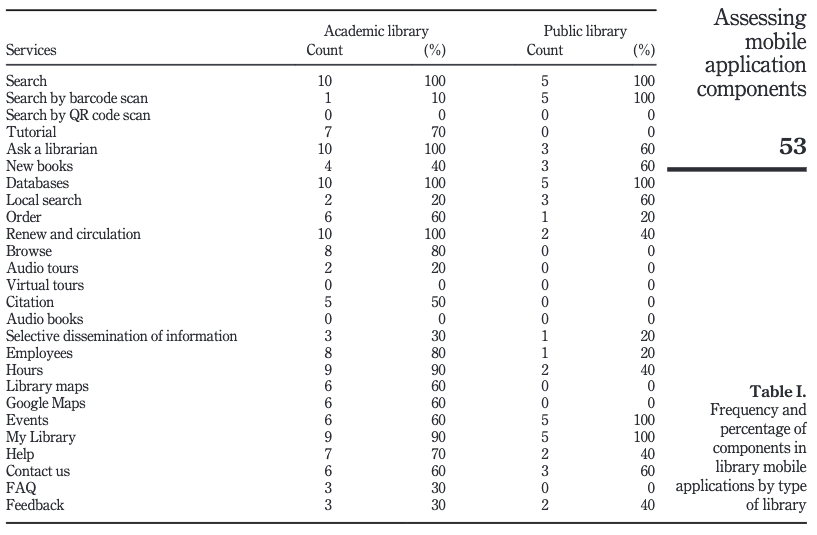
\includegraphics[width = \textwidth, height = \textheight, keepaspectratio]{assets/img/accessing_mobile_application_components_table_1.png}
        \caption{Frequency and percentage of components in library mobile applications by type of library \protect\citeA{mansouri_soleymani_asl_2019}}
        \label{fig:freq_and_per_comp_lib_mob_app}
    \end{figure}
    \paragraph{}
    The above (Figure ~\ref{fig:freq_and_per_comp_lib_mob_app}) is from Mansouri and Soleymani's study. In summary, it breaks down all services found in the library mobile applications they reviewed, and how often they were used. The "Public library" column is irrelevant in this report. This is a great example of a model for features that are used in the field already. We will break down all relevant features and provide comments on each.
    \paragraph{Search (by barcode/QR code scan)}
    We assume these features refer to a user's ability to search the library catalog. At the time of this writing, this is a feature we do not plan on implementing in the \appname app. However, it is an important one, as according to this study, all existing library apps reviewed had this features. We believe for a mobile app that is intended to be a replacement for a desktop website to be successful, it must provide the most common services provided by its desktop website counterpart.
    \paragraph{Tutorial}
    We assume this feature refers to a visual tutorial provided within the mobile app that teaches new users how to use said mobile app. The study found that 70\% of library mobile apps had this feature. A tutorial allows new users to get a better understanding of how to use a platform. Without a tutorial, many new users may be lost, therefore rendering the mobile app useless for them. As of this writing, we had not considered this feature, but have since taken it under consideration.
    \paragraph{Ask a librarian}
    We assume this feature refers to a user's ability to submit questions to a librarian. The study found all library mobile apps included this feature. We plan to implement a similar feature: the library chat.
    \paragraph{Audio books}
    We assume this features refers to a user's ability to search and listen to audio books. We have discussed this with our advisor, who says the WPI library has a lot of audio books in its database. As of this writing, we have dismissed the idea of implementing this feature. As this study shows, it seems that others have too. We do feel that this features would be interesting, but clearly, according to the study, there has been no adoption (among the study's data set).
    \paragraph{Hours}
    Straight-foward features that provides users with library hours. We plan on implementing this feature in the \appname app.
    \paragraph{Events}
    We assume this feature refers to a user's ability to view library events and/or a calendar. The study found that 90\% of library mobile apps have this feature. We plan on implementing it as well. If we are to produce a library mobile app with many other features, it is possible that users will prefer the app to the desktop website. It would be silly to not include such a useful feature such as a calendar of library events. Users should not have to use a separate service.
    \paragraph{FAQ/Feedback}
    It surprised us that only 30\% of library mobile apps have this feature. The whole point of this project is to provide students easier access to the WPI library's various services. As a team of four (including our advisor), it is impossible for us to make a perfect product. This would really apply to any team size because there is always some disconnect between what the developers think consumers want, and what the consumers actually want. We plan on implementing a platform for users of the \appname app to provide feedback on their experience.

    \begin{itemize}
        
        \item
        The use of mobile apps is increasingly widespread, and much effort is put into testing these apps to make sure they behave as intended.To reduce this effort, and thus the cost of mobile app testing, we propose AppTestMigrator, a technique that allows for migrating test cases between apps with similar features. The intuition behind AppTestMigrator is that many apps share similarities in their functionality, and these similarities often result in conceptually similar user interfaces (through which that functionality is accessed). Typical examples of this situation are apps in the same category, apps developed based on the same specification, and different versions of the same app. In all these cases, the burden of writing test cases can be reduced by migrating test cases written for an app to another, similar app. Given a test case for an app (source app) and a second app (target app), AppTestMigrator attempts to automatically transform the sequence of events in the test for the source app to events that can be consumed by the target app.\cite{Test_Migration}
        \item
        Mobile apps are used on a daily basis to perform a number of tasks such as reading the news, accessing social media, and shopping. It is therefore important to thoroughly test these apps, to gain confidence that they behave as intended when used in the field. Unfortunately, developing test cases for an app, as for any software system in general, is extremely expensive. We believe that the cost of testing mobile apps can be considerably reduced by considering similarities between apps and reusing test cases across similar apps. \cite{Test_Migration}
        \item
        We presented AppTestMigrator, a technique that aims to decrease the cost of app testing by leveraging the similarities between GUIs of different yet related apps and performing test migration—reusing and adapting test cases among such apps. AppTestMigrator can be used in all those situations in which different apps share similarities that result in conceptually similar GUIs. We implemented a prototype of AppTestMigrator that supports Android apps and tests written using the Espresso framework, and we have used our prototype to evaluate our approach on four randomly selected shopping list apps from the Google Play Store. We believe that our results, although still preliminary, show clear evidence of the potential usefulness of our approach. In future work, we will first perform additional experiments to validate our findings and guide future research. Second, we will extend the technique so that it can migrate test oracles (i.e., assertions), in addition to events. Finally, we will investigate large scale applications of our approach, in the context of a database of apps and tests for these apps. Developers could submit their apps to the database, which would analyze them, look for similar apps, migrate the tests from these apps, and return all the tests that were successfully migrated. If successful, this could result in a sort of store that operates in parallel to the app store. \cite{Test_Migration}
    \end{itemize}
    
    
\section{State of the Art}
    \paragraph{}
    Throughout the years, app development has improved in both efficiency, quality, and accessibility. As a result, library apps - as well as similar learning-based apps - have improved in these criteria congruently. One feature of modern day mobile applications is an emphasis integration with other relevant software. For example, in reference to the Libris CampusM Mobile App, an article writes: "The flexibility of the app enables it to be integrated with learning management systems such as Blackboard®, Canvas, and Moodle™"\cite{campusM}. This cross-platform paradigm is quintessential in applications which were build to service existing technologies. State of the art library mobile applications then, integrate with existing programs and databases. One papers describes the origins of a library mobile app; "A number of libraries gradually sensed this trend and combined their services with mobile technology to created so-called Mobile Library or M-Library." \cite{design_and_impl}
    \paragraph{}
    In addition to be highly integrated with existing technology, state of the art mobile applications utilize technologies built into smartphones in order give users the best possible experience. One papers states, "The behavior of smartphone apps is driven by input from sensors such as GPS, microphone, or camera"  \cite{}. State of the art library applications utilize the technology provided by mobile phones in order to maximize their utility. For example, a library app might use the camera in order to scan bar codes. Furthermore, a library application could utilize the GPA technology to inform users with their distance from the library. Essentially, state of the art apps, including library apps, utilize the state of the art technology features on smartphones.
    \paragraph{}
    Another feature of modern technology, particularly software, is change. State of the art application are dynamic entities; they improve with time and require consistent maintenance. One author writes, "Thus, to keep the software and its data safe, software developers perform continuous testing of the product in its operational phase and release software upgrades or software updates/patches to fix any uprising issue and to improve it.\cite{Reliability_modeling}.  Essentially, state of the art software, mobile applications specifically, including library applications, are upgraded, maintained and modified on a regular basis.
    \paragraph{}
    Yet another feature of state of the art software is the it's ability to provide value in multiple ways. State of the art tools not only provide useful services to the clients, but also provide the client with value. With respect to library application specifically, this means the software is designed such that data can be collected from the users to exponentially improve the software. One author notes, "This indicated that Mobile Library has become a vital resource for learners to acquire knowledge"\cite{given_one}.  Essentially, state of the art software is designed such that developers can improve the experience for users exponentially, by collecting valuable data from its users.  
    
    %%List here is just for information purposes. Text above is the actual thing
    
    % \begin{itemize}
    
    %     \item
    %     "The flexibility of the app enables it to be integrated with learning management systems such as Blackboard®, Canvas, and Moodle™" \cite{campusM}
    %     \item
    %     "Since the app runs on library-developed open-source software, feedback from academic users during the pilot program – currently running until August 31 – will also help develop and improve new functionality in the app, which will benefit all library users." \cite{NYU_Library}.
    %     \item
    %     "Since the app runs on library-developed open-source software, feedback from academic users during the pilot program – currently running until August 31 – will also help develop and improve new functionality in the app, which will benefit all library users." \cite{NYU_Library}.
    %     \item 
    %     "The behavior of smartphone apps is driven by input from
    %     sensors such as GPS, microphone, or camera", 
    %     "First, we fuzz (alter) the log in a semantically-meaningful way: by applying 
    %     principled transformations (e.g., changing GPS coordinates
    %     or navigation speed), a new input log is constructed, which
    %     represents a new test case. Second, we use the log captured
    %     in app A to test an app B which offers similar functionality,
    %     e.g., GPS navigation or image recognition"
    %     "For example, GPS allows apps such as Yelp to provide location-aware services; the camera allows image matching apps like Google Goggles to provide search-by-picture features; the Shazam app can help recognize an ambient song by using the microphone."
    %     \cite{FuzzyAndCross}
    %     \item
    %     With the unceasing advancement of mobile technologies, mobile devices developed rapidly. Thus, learning activities could be proceeded anytime and anywhere (Lai et al. , 2014). Wang et al. (2012) indicated that, with the popularization of 3G mobile technologies, more people gained access to internet to view web site, receive and send e-mails and read e-books with smartphones and tablet PCs on metro, bus or train. It could be inferred that learning activities no longer limit to classroom or scheduled time. By combining mobile devices and wireless technology, learning guidance and feedbacks could be given according to learners' learning situations and learning environment (Huang et al. , 2014).

    %     A number of libraries gradually sensed this trend and combined their services with mobile technology to created so-called Mobile Library or M-Library. In fact, the concept of Mobile Library or M-Library was brought up by scholars when PDAs were still in development. For instance, Janet (2009) adapted mobile technology and combined PDA with library orientation and collection search services. However, at that time, mobile devices and wireless technology were not mature and popular.
        
    %     "Recently, mobile technology combined with mobile devices has become an important information collecting channel. A greater number of students and teachers also use tablet PCs and smartphone to search for e-journals, e-books and other e-resources (Parsons, 2010). Therefore, numerous libraries introduced mobile technology in library services and developed mobile information systems compatible to mobile devices in order to allow their users quickly search for desired information (Wang et al. , 2012). This indicated that Mobile Library has become a vital resource for learners to acquire knowledge."
    %     "Ten participants reported that it was easier to search the library catalog using the laptop.They explained that they were familiar with the interface of web OPACs, and moreinformation was displayed on the computer screen than the tablet screen"
    %     "Some participants reported that they would use the smartphone app to search librarycatalogs when it was inconvenient to use laptops or desktop computers, such as on the bus or in classroom"
    %     \cite{given_one}
       
    % \end{itemize}
    
\section{Relation to the Larger Problem Area}
    \paragraph{}
     As the world becomes more digitized, and tools once only accessible in person are made accessible via the internet, projects such as this become increasingly relevant. One particular field in which modernization is fast-growing is mobile development. Specifically, mobile development with respect to the virtualization of already existing tools. These applications include mobile apps to make delivery placements for food, mobile applications to handle transportation, and generally any service that can be digitized. "The open-source community is helping to rapidly advance mobile Web application development. To date, no less than eighteen different mobile frameworks exist just for the iPhone"\cite{MobiOne}. Mobile application is one of the broadest and most widely used examples of the digitization of the modern world. 
     
     \paragraph{}
     A number of factors explain this trend towards digitization via mobile applications. Firstly is the decreased cost. A major advantage of software is its repeatably. If software if developed once, it could be re-implemented as many times as desired with virtually no additional cost. Furthermore, mobile applications save users a significant amount of time; virtually any good or service is a few clicks away. Another factor in the popularization of mobile applications is the popularity of smart phones. One source writes: "This time next year we expect the mobile Web to have matured significantly as smartphones get cheaper and more diverse, and desktop developers spend more energy creating applications for the computer in your pocket,"\cite{MobiOne}. As smartphones become more popular, digitization implemented with this software will become more popular, leading to the further popularization of smart phones. The result, then, would be a positive feedback loop between smartphones and mobile apps. 
     
     \paragraph{}
     Application development with respect to library services in particular, is a fast-growing niche. One author writes, "Recently, mobile technology combined with mobile devices has become an important information collecting channel. A greater number of students and teachers also use tablet PCs and smartphone to search for e-journals, e-books and other e-resources"\cite{pu_chiu_chen_huang_2015}
     In essences, library features become a particularly fruitful avenue for the area of the modernization and digitization of existing tools. This trend can be attributed to the data-driven services libraries provide. Libraries provide excessive amounts of data, giving developers solid materials to work with. Furthermore, libraries tend to be affiliated with higher education - often a University for example - which further increases the inclination of software developers, often affiliated with these places of higher learning, to develop mobile applications for these institutes. 
     \paragraph{}
     Furthermore, mobile library specific application development has been proven to be highly for library administrators. This is because mobile apps serve not just the function of aiding its users in whatever tasks its been designed to aid with, but also because they can be regarded as a data collection tool for individuals overseeing the institute with which the application is connected. Regarding the usage of library application to collect data, one author writes, "Recently, mobile technology combined with mobile devices has become an important information collecting channel. A greater number of students and teachers also use tablet PCs and smartphone to search for e-journals, e-books and other e-resources  (Parsons,  2010).  Therefore,  numerous  libraries  introduced  mobile technology in library services and developed mobile information systems compatible to mobile devices in order to allow their users quickly search for desired information"\cite{pu_chiu_chen_huang_2015}. Mobile apps allow library administrators to get nearly instant feedback with regards to the various services and features offered by the library, making it a useful tool for growing and developing libraries and library services. 
    
    
    % \begin{itemize}
    %     \item 
    %     "The open-source community is helping to rapidly advance mobile Web application development. To date, no less than eighteen different mobile frameworks exist just for the iPhone. Yet few mobile Web developers know of them and their rich user interface capabilities and smart device features. MobiOne is introducing Community Insights, an integrated feature that brings together real time news and information about mobile Web frameworks with numerous examples that can be instantly loaded into the MobiOne iPhone and Palm Pre emulators for evaluation. "This time next year we expect the mobile Web to have matured significantly as smartphones get cheaper and more diverse, and desktop developers spend more energy creating applications for the computer in your pocket," said Maher Masri, president and CEO of Genuitec. "Mobile devices are becoming more prevalent and as the market grows, software developers will be armed for success with powerful tools like MobiOne.""\cite{MobiOne}
        
    %     \item
    %     There exists a trend towards mobile computing. "Gradually, many libraries sense this trend and start to ponder on methods of providing innovative services by using mobile technology". Mobile innovative services of library means that a library utilizes mobile technology to allow is readers view,search and obtain library services without being limited by time and place (Chang,2013) \cite{pu_chiu_chen_huang_2015}. In summary, libraries are attempting to offer mobile applications for their services. We want to do exactly that. We want an application that students can use wherever and whenever to access library services.
        
    %     \item
    %     "Recently, mobile technology combined with mobile devices has become an important information collecting channel. A greater number of students and teachers also use tablet PCs and smartphone to search for e-journals, e-books and other e-resources  (Parsons,  2010).  Therefore,  numerous  libraries  introduced  mobile technology in library services and developed mobile information systems compatible to mobile devices in order to allow their users quickly search for desired information(Wanget al., 2012). This indicated that Mobile Library has become a vital resource for learners to acquire knowledge" \cite{pu_chiu_chen_huang_2015}.
    %     \item
    %     Found in a study by a team from San Agustin University's Computer Science department in Peru, and among 163 surveyed students, those students mostly utilize academic apps that assist in making their academic workload easier and more efficient to handle. These such apps include: GeoGebra, Mathway, Kahn Academy, Duolingo, Symbolab, and numerous others. As we delve into the concept of creating a more ease of access system for academic resources here at WPI, this study shows just what students are wanting from mobile apps, convenience.\cite {Educational_Apps}
    % \end{itemize}
    
    \section{Closing Thoughts}
    \paragraph{}
    More and more are mobile devices being utilized even in an academic context. There is a growing need for resources in higher education. Easy access to academic library services is just one of these many needs. As this need is still in its infancy, not much is known about mobile library applications specifically. More so, much is known about the development of mobile applications and the requirements of a mobile library app, based on the feedback from students. However, we have not seen these applications implemented frequently. With that said, observed common patterns among the state of the art library application we analyzed. One pattern was that the application was integrated with the already existing library features; as opposed to developing features from scratch, the built on the existing tools offered by libraries. Furthermore, they were dynamic. They were designed such that they could be updated in accordance to how the clients used them; they provided developers with data to upgrade and improve the experience for the users. The development of these applications tracks with the trend of the modern world towards digitization. This trend can be attributed to the application's aforementioned  ability to be  upgraded in accordance to the user's needs and desires, largely from the data returned by the app to the administrators and developers. The digitization of library tools saves time and has proven to be beneficial for both administrators and users alike.